\documentclass[11pt, english]{report}
\usepackage{graphicx}
\usepackage[colorlinks=true, linkcolor=blue]{hyperref}
\usepackage[english]{babel}
\selectlanguage{english}
\usepackage[utf8]{inputenc}
\usepackage[svgnames]{xcolor}
\usepackage{url}
\usepackage{hyperref}
\usepackage{float}
\usepackage{longtable}
\usepackage[toc]{glossaries}
\usepackage{amsmath}
\usepackage{amssymb}

\usepackage{algpseudocode}
\usepackage{algorithm}
\usepackage{csquotes}
\usepackage{booktabs}

\usepackage{listings}

\newcommand{\R}{\mathbb{R}}


\usepackage{listings}
\usepackage{afterpage}
\pagestyle{plain}


\definecolor{dkgreen}{rgb}{0,0.6,0}
\definecolor{gray}{rgb}{0.5,0.5,0.5}
\definecolor{mauve}{rgb}{0.58,0,0.82}
\usepackage{biblatex}
\bibliography{ref.bib}

%\lstset{language=R,
%    basicstyle=\small\ttfamily,
%   stringstyle=\color{DarkGreen},
%    otherkeywords={0,1,2,3,4,5,6,7,8,9},
%    morekeywords={TRUE,FALSE},
%    deletekeywords={data,frame,length,as,character},
%    keywordstyle=\color{blue},
%    commentstyle=\color{DarkGreen},
%}

\lstset{frame=tb,
language=R,
aboveskip=3mm,
belowskip=3mm,
showstringspaces=false,
columns=flexible,
numbers=none,
keywordstyle=\color{blue},
numberstyle=\tiny\color{gray},
commentstyle=\color{dkgreen},
stringstyle=\color{mauve},
breaklines=true,
breakatwhitespace=true,
tabsize=3
}


\usepackage{here}


\textheight=21cm
\textwidth=17cm
%\topmargin=-1cm
\oddsidemargin=0cm
\parindent=0mm
\pagestyle{plain}

\usepackage{color}
\usepackage{ragged2e}

\global\let\date\relax
\newcounter{unomenos}
\setcounter{unomenos}{\number\year}
\addtocounter{unomenos}{-1}
\stepcounter{unomenos}
\gdef\@date{ Course \arabic{unomenos}/ 2019}

\makeglossaries
 
\newglossaryentry{eternity}
{
    name=ETERNITY: FUNCTIONS,
    description={It stands for the name of both the project and the product, unless otherwise stated}
}

\begin{document}

\begin{titlepage}

\begin{center}
\vspace*{-1in}
\begin{figure}[htb]
\begin{center}

\includegraphics[width=8cm]{logo}
\end{center}
\end{figure}
\begin{Large}
\textbf{SOEN 6011 - Software Engineering Processes} \\
\end{Large}
\vspace*{0.1in}
Summer 2019\\
\vspace*{0.5in}
\begin{Large}
\textbf{Scientific Calculator-  ETERNITY: FUNCTIONS} \\
\end{Large}
\vspace*{0.4in}
\begin{large}
Project Report\\
\end{large}
\vspace*{0.2in}
\begin{Large}
\textbf{Deliverable 3} \\
\end{Large}
\vspace*{0.3in}
\begin{large}
Presented to \\
\vspace*{0.1in}
Instructor: PANKAJ KAMTHAN 
 \\
\end{large}
\vspace*{0.3in}
\rule{80mm}{0.1mm}\\
\vspace*{0.1in}
\begin{large}
By \\
Prashanthi Ramesh\\ 
\vspace*{0.3in}
\date{\normalsize\today} 

\end{large}
\end{center}
\end{titlepage}

\newcommand{\CC}{C\nolinebreak\hspace{-.05em}\raisebox{.4ex}{\tiny\bf +}\nolinebreak\hspace{-.10em}\raisebox{.4ex}{\tiny\bf +}}
\def\CC{{C\nolinebreak[4]\hspace{-.05em}\raisebox{.4ex}{\tiny\bf ++}}}

\tableofcontents
\newpage
\chapter{Source Code Review}

Eternity Function F1: arccos(x)  developed by Himansi Patel

\section{Manual Code Review}

\subsubsection{Use of Static Methods}

Non-static methods\cite{codereview1} defined in classes HelperFunction and ArccosFunction - calculatePI(), calculateFactorial(int number), calculatePower(double base, int exponent), arccos(double num) can be declared static.

\begin{figure}[H]
  
  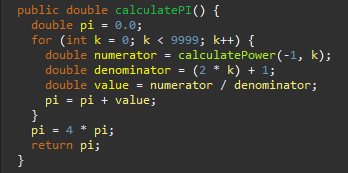
\includegraphics[width=0.6\textwidth]{codereview/staticmethod.PNG}
  \centering
  \caption{ A non-static method in HelperFunction class that can be declared as static
}
\end{figure}

\begin{itemize}
    \item Methods are declared static as they do not hold the state of an object of the class
\end{itemize}

\subsubsection{Missing Javadoc Comments}

Unit test methods in classes ArccosTest and HelperFunctionTest can include javadoc comments to quickly understand the purpose of the tests.

\begin{figure}[H]
  
  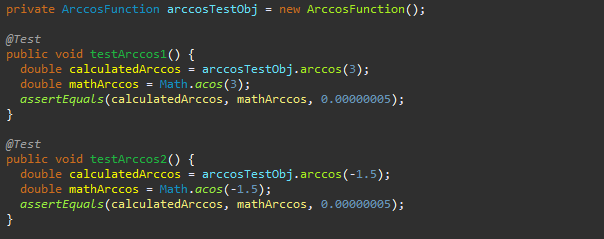
\includegraphics[width=1\textwidth]{codereview/javadoccommentmissing.PNG}
  \centering
  \caption{ Missing comments in Unit Test Methods
}
\end{figure}

\subsubsection{Naming Conventions}

Unit test methods in classes ArccosTest and HelperFunctionTest can include self-descriptive method names to quickly understand the purpose of the tests.

\begin{figure}[H]
  
  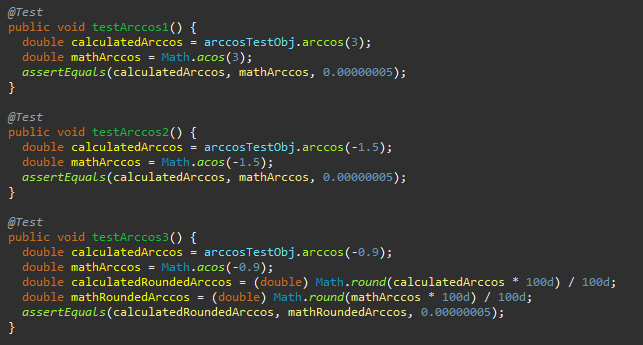
\includegraphics[width=0.9\textwidth]{codereview/testcasemethodnames.PNG}
  \centering
  \caption{ Method names that can be changed to self-descriptive names
}
\end{figure}

\section{Automatic Code Review}

\begin{itemize}
    \item For automatic source code review CheckStyle\cite{checkstyle} plugin for eclipse IDE was used.
    \item The Google Checks configuration was used to check if there are any deviations from the defined set of coding rules.
    \item The analysis showed no violations in the source code.
\end{itemize}


\subsubsection{CheckStyle Plugin}

Checkstyle inspects your Java source code and pointing out items that deviate from a defined set of coding rules.

\begin{figure}[H]
  
  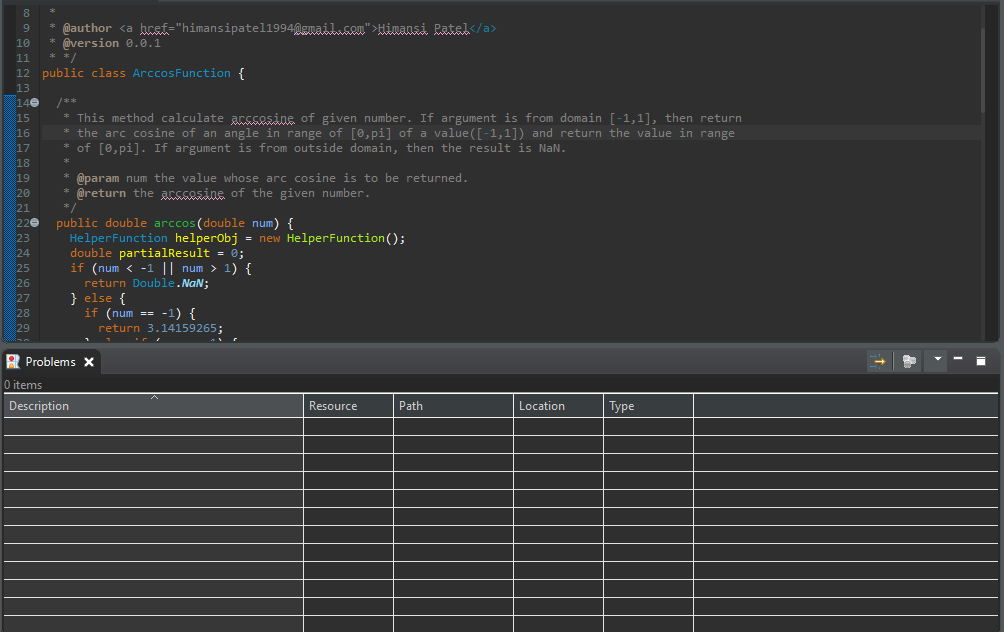
\includegraphics[width=1\textwidth]{codereview/googlecheckstyle.PNG}
  \centering
  \caption{ No violations generated by CheckStyle Plugin in Eclipse IDE
}
\end{figure}



\chapter{Testing}

Eternity Function F2: tan(x) developed by Nirav Patel

\section{Environment}

\begin{itemize}
    \item Unit tests are created in Java in a separate project or separate source folder to keep the test code separate from the real code.
    \item The standard convention from the Maven and Gradle build tools is to use:\\ 
    
    src/test/java - for test classes
\end{itemize}
 

\section{Procedure}

All Unit test cases created by the developer are working fine.

\begin{figure}[H]
  
  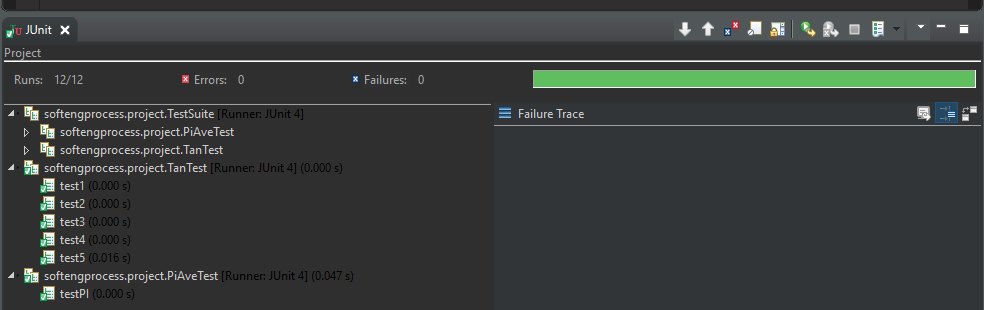
\includegraphics[width=1\textwidth]{testing/unittestspassed.PNG}
  \centering
  \caption{ Test cases are passed in JUnit\cite{unittest} in Eclipse IDE
}
\end{figure}


\begin{figure}[H]
  
  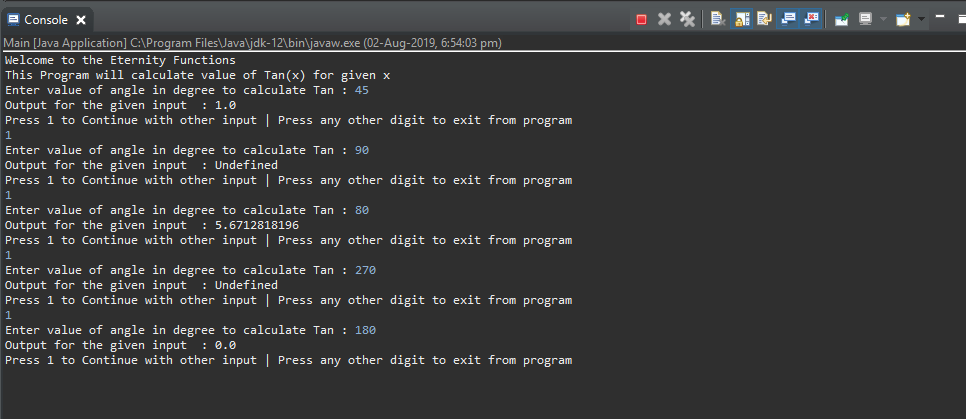
\includegraphics[width=1\textwidth]{testing/testedfortestcases.PNG}
  \centering
  \caption{ Test Cases that pass using JUnit are verified
}
\end{figure}

\begin{figure}[H]
  
  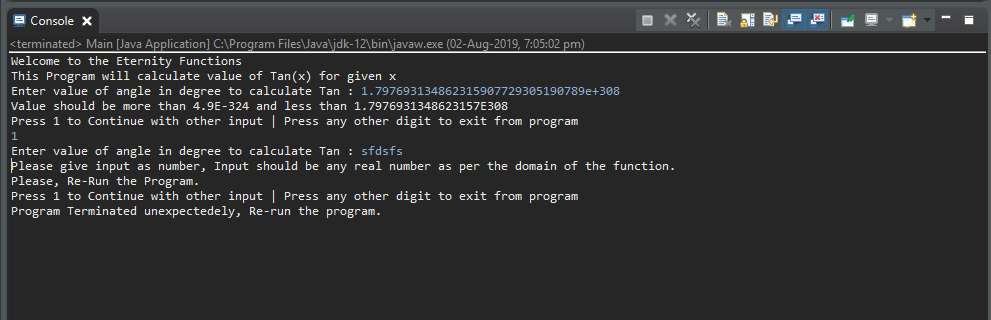
\includegraphics[width=1\textwidth]{testing/invalidrangeinput.PNG}
  \centering
  \caption{ Test for valid input within the specified range in the requirement document
}
\end{figure}

Apart from the test cases written by the developer, I have performed the following tests. 
\vspace*{1.5in}
\begin{table}[!htp]
\centering

\caption{Test Results}
\vspace*{0.2in}
\begin{tabular} {@{}|l|l|l|l|l|l|l|@{}}

\toprule

\multicolumn{1}{|c|}{ID} & \multicolumn{1}{c|}{Date} &  \multicolumn{1}{c|}{Input(degree)} & \multicolumn{1}{c|}{Expected Output}  & \multicolumn{1}{c|}{Actual Output} & \multicolumn{1}{c|}{\begin{tabular}[c]{@{}c@{}}State\\ (Pass/Fail)\end{tabular}} \\ \midrule


1          & 2 August, 2019                           &   0                       & 0                                   & 0                        & Pass                                                                             \\ \midrule


2          & 2 August, 2019                             &   -360                   & 0 & 0 & Pass                                                 \\ \midrule

3                                   & 2 August, 2019    &  -45                    & -1 & -1 & Pass                                                 \\ \midrule


4       & 2 August, 2019                                &    -90                  & Undefined & Undefined & Pass                                                 \\ \midrule

5              & 2 August, 2019                         &   -80                   & -5.67128 & -5.67128 & Pass                                                 \\ \midrule



6             & 2 August, 2019                          &    -270                  & Undefined & Undefined & Pass                                                 \\ \midrule



7              & 2 August, 2019                         &     -180                & 0 & 0 & Pass                                                 \\ \midrule

8           & 2 August, 2019                            &     53                 & 1.32704 & 1.32704 & Pass                                                 \\ \midrule

9          & 2 August, 2019                             &     99                 &-6.31375 & -6.31375 & Pass                                                 \\ \midrule


10          & 2 August, 2019                             &  -99                    & 6.31375 & 6.31375 & Pass                                                 


\\ \bottomrule
\end{tabular}
\end{table}


\appendix
\chapter{GitHub}
\section{Individual GitHub Link}
https://github.com/PrashanthiRamesh/SOEN-6011-Project-Calculator/

\section{Source Code Review Github Link of Himansi Patel}
https://github.com/Himansipatel/SOEN-6011-Team-H-Himansi/

\section{Testing Github Link of Nirav Patel}
https://github.com/niravjdn/SOEN-6011-Project-Team-H-Nirav/

\section{Team GitHub Link}
https://github.com/niravjdn/SOEN-6011-Project/


\printbibliography

\printglossary

\end{document}